% Chapter 6
\chapter{Feasibility Study}
\label{ch:evaluation}

\section{Study Overview}
The evaluation follows a feasibility study design to check whether the multimodal AI-driven adaptation pipeline works end to end under realistic interaction traces, and whether it does so in a way that is useful for accessibility. Concretely:
\begin{enumerate}
  \item \textbf{Adaptation validity:} Does the backend return schema-valid adaptation objects across different profiles and modalities?
  \item \textbf{Accessibility relevance:} Do adaptations match user needs (motor, visual, hands free) and observed errors (for example \texttt{miss\_tap}, \texttt{slider\_miss})?
  \item \textbf{Latency:} What is end-to-end response time (p50/p90/max) under the chosen backend configuration?
\end{enumerate}

\section{Methodology}
\paragraph{Profiles and runs.}
Six user profiles (P0--P5) were selected to cover baseline, single-need, and combined needs:
\begin{itemize}
  \item \textbf{P0 (Baseline):} No specific accessibility needs.
  \item \textbf{P1 (Motor):} Larger touch targets; keyboard preferred.
  \item \textbf{P2 (Visual):} Larger font and higher contrast preferred.
  \item \textbf{P3 (Hands free):} Voice and gesture preferred.
  \item \textbf{P4 (Motor + Hands free):} Combined motor support and voice preference.
  \item \textbf{P5 (Visual + Motor):} Combined visual and motor support.
\end{itemize}
For each profile, two runs were executed to allow a small history to build. Each run used the same seven-event sequence (14 events per profile, 84 total); see Table~\ref{tab:user-profile-mapping}.

\begin{table}[h]
\centering
\caption{User profile mapping for evaluation runs.}
\begin{tabular}{ll}
\toprule
\textbf{Profile} & \textbf{Declared needs} \\
\midrule
P0 & Baseline (no declared needs) \\
P1 & Motor, keyboard preferred \\
P2 & Visual, larger font \\
P3 & Hands free preferred, voice modality \\
P4 & Motor + Hands free, voice modality \\
P5 & Visual + Motor, voice modality \\
\bottomrule
\end{tabular}
\label{tab:user-profile-mapping}
\end{table}

\paragraph{Event suite.}
The suite mixes errors and successful attempts across modalities and targets (lamp, thermostat, lock):
\begin{itemize}
  \item \texttt{miss\_tap} on buttons (lamp, lock),
  \item \texttt{slider\_miss} with overshoot (thermostat),
  \item \texttt{voice} commands (turn on, unlock, adjust),
  \item \texttt{gesture} inputs (point/select).
\end{itemize}
This combination triggers typical accessibility challenges (tap precision, slider control, and mode switching).

\paragraph{Backend configuration and metrics.}
All traces used the MA-SIF (balanced) configuration (Table~\ref{tab:ma-sif-config}). Each event’s response was checked for schema validity; the classification path and client-side latency (p50/p90/max) were logged. Analysis scripts flatten JSONL logs to CSV and compute objective metrics.

\begin{table}[htb]
\centering
\caption{MA-SIF (balanced) agent configuration.}
\label{tab:ma-sif-config}
\begin{tabular}{lcccc}
\toprule
\textbf{Agent} & \textbf{Model} & \textbf{Thinking budget} & \textbf{Temperature} & \textbf{Timeout (s)} \\
\midrule
UI         & gemini-flash-lite & 0   & 0.2 & 15 \\
Geometry   & gemini-flash-lite & 0   & 0.2 & 15 \\
Input      & gemini-flash-lite & 0   & 0.2 & 15 \\
Validator  & gemini-flash      & -1  & 0.3 & 30 \\
\bottomrule
\end{tabular}
\end{table}

\paragraph{Hardware and Environment:}
All experiments in this thesis were executed on a single development machine in a controlled home environment (none to low network contention). Latency is end-to-end from event send to response received on the client.
Hardware configuration:
\begin{itemize}
    \item \textbf{Hardware:} MacBook Pro, M1 Max 10-core CPU, 32\,GB RAM
    \item \textbf{Software:} macOS 15.6 (Sequoia), Python 3.9+
    \item \textbf{Environment:} Localhost + Gemini external API calls
\end{itemize}

\paragraph{Operational definitions.}
\textbf{Schema-valid} means the response conforms to the adaptation schema (valid action names, parameters in bounds, resolvable UI targets, and consistency checked by the Validator). \textbf{Latency} is measured as $\Delta t = t_{\text{recv}} - t_{\text{send}}$.

\paragraph{Objective scoring rules.}
All quality metrics are computed deterministically from the logs using fixed contracts and allowed actions. Two lookup tables are used:

\noindent\textbf{(i) Action $\rightarrow$ Accessibility Category}

\begin{table}[H]
\centering
\small
\renewcommand{\arraystretch}{1.3}
\caption{Mapping of adaptation actions to accessibility categories.}
\begin{tabular}{ll}
\toprule
\textbf{Action} & \textbf{Accessibility Category} \\
\midrule
\texttt{increase\_button\_size}      & Motor \\
\texttt{increase\_button\_border}    & Motor \\
\texttt{increase\_slider\_size}      & Motor \\
\texttt{adjust\_spacing}             & Motor \\
\texttt{increase\_font\_size}        & Visual \\
\texttt{increase\_contrast}          & Visual \\
\texttt{switch\_mode} (\texttt{voice} or \texttt{gesture}) & Hands-free \\
\texttt{trigger\_button} (from voice intent) & Hands-free \\
\bottomrule
\end{tabular}
\end{table}

\noindent\textbf{(ii) Error Event $\rightarrow$ Acceptable Corrective Adaptations}

\begin{table}[H]
\centering
\small
\renewcommand{\arraystretch}{1.3}
\caption{Mapping of error events to acceptable corrective adaptations.}
\begin{tabular}{ll}
\toprule
\textbf{Error Event} & \textbf{Acceptable Corrective Adaptations} \\
\midrule
\texttt{miss\_tap} &
\begin{tabular}[t]{@{}l@{}}
\texttt{increase\_button\_size}, \texttt{increase\_button\_border}, \\
\texttt{adjust\_spacing}, \texttt{switch\_mode:voice}
\end{tabular} \\
\texttt{slider\_miss} &
\begin{tabular}[t]{@{}l@{}}
\texttt{increase\_slider\_size}, \texttt{adjust\_spacing}
\end{tabular} \\
\texttt{voice} (command) &
\begin{tabular}[t]{@{}l@{}}
\texttt{switch\_mode:voice}, \texttt{trigger\_button} (if intent clear)
\end{tabular} \\
\texttt{gesture} (point/select) &
\begin{tabular}[t]{@{}l@{}}
\texttt{switch\_mode:gesture}, \texttt{trigger\_button} (if intent clear)
\end{tabular} \\
\bottomrule
\end{tabular}
\end{table}

These tables are grounded in the schema and rule-based fallbacks, which makes the assessment replicable and objective.

\section{Accessibility and Design Quality}
\label{sec:objective-quality}
This section reports effectiveness before latency, using objective, log-derived metrics. Effectiveness is assessed by quantifying how well the adaptation pipeline produces accessibility-relevant, profile-aligned, and internally coherent UI changes in response to realistic interaction traces. Metrics such as Profile–Action Alignment (PAA), Error to Response Appropriateness (ERA), Mode Enablement for Hands free (MEH), and Design Coherence Index (DCI) are computed directly from adaptation logs, enabling reproducible and objective evaluation. These results provide a detailed view of the system’s accessibility impact and personalization quality prior to analyzing performance characteristics such as latency.

\subsection{Profile–Action Alignment (PAA)}
\textbf{Definition.}
PAA is the share of accessibility actions whose category matches the active profile’s needs (motor, visual, hands free):
\[
\mathrm{PAA} = \frac{\#\{ \mathrm{cat}(a)\in \mathrm{needs}(p)\}}{\#\{\text{accessibility actions}\}} \times 100\%.
\]
\textbf{Result.}
Across non baseline profiles (P1–P5), and using the top five actions per profile, PAA is approximately \textbf{55\%}. Combined-need profiles show higher alignment (P4 80.00\%, P5 77.42\%) than single-need profiles that are underrepresented by the event suite (P2 34.69\%, P3 28.00\%); see Table~\ref{tab:obj-metrics}.

\subsection{Error to Response Appropriateness (ERA)}
\textbf{Definition.}
ERA is the share of error or modality events that received at least one acceptable corrective adaptation:
\[
\mathrm{ERA} = \frac{\#\{\text{error events with }\geq 1 \text{ corrective adaptation}\}}{\#\{\text{error events}\}} \times 100\%.
\]
\textbf{Result.}
ERA ranges from \textbf{50.00\%} to \textbf{64.29\%} per profile (for example P5 64.29\%), indicating that about one half to two thirds of these events contain a corrective action from the predefined set (Table~\ref{tab:obj-metrics}).

\subsection{Mode Enablement for Hands free (MEH)}
\textbf{Definition.}
MEH is the share of events in which a hands free path is explicitly enabled or used (\texttt{switch\_mode:voice|gesture} or voice \texttt{trigger\_button}).

\[
\mathrm{MEH} = \frac{\#\{\text{events with \texttt{switch\_mode:voice|gesture} or accepted \texttt{trigger\_button} via voice}\}}{\#\{\text{events}\}} \times 100\%.
\]

\textbf{Result.}
MEH equals \textbf{57.14\%} for hands free profiles P3 and P4, indicating frequent enablement of non touch paths; values are lower for profiles where hands free is not a primary need (Table~\ref{tab:obj-metrics}).

\subsection{Design Coherence Index (DCI)}
\textbf{Definition.}
DCI quantifies the absence of contradictions and duplicates within a single response:
\[
\mathrm{DCI} = 1 - \frac{\#(\text{conflicts}+\text{duplicates})}{\#\text{suggestions}}.
\]
\textbf{Result.}
DCI is high across profiles (mean $\approx$\textbf{0.995}), which indicates internally consistent, non redundant suggestions (Table~\ref{tab:obj-metrics}).

\subsection{Global accessibility share and WCAG coverage}
Overall, \textbf{97.51\%} of all actions are accessibility targeted (352/361), see Table~\ref{tab:overall-accessible-share}. The policy level coverage in Table~\ref{tab:wcag-coverage} shows that proposed adaptations address SC~2.5.5 (Target Size), SC~1.4.3 (Contrast), and SC~1.4.4 (Resize Text). This is coverage, not a conformance audit.

\subsection{Motor Benefit Proxy (Fitts law, analytic)}
\textbf{Rationale:}
When targets are enlarged by a factor \(s\) (for example \(s{=}1.5\)), the Fitts law index of difficulty changes from \(\log_2(\frac{D}{W}+1)\) to \(\log_2(\frac{D}{sW}+1)\).
For representative \(D/W\) ratios, a 1.5\(\times\) size increase yields the following theoretical reductions:

\begin{table}[h]
\centering
\caption{Fitts law proxy: relative reduction in index of difficulty for \(s{=}1.5\).}
\begin{tabular}{lrrrrr}
\toprule
\(D/W\) & 2 & 4 & 8 & 12 & 16 \\
\midrule
Reduction (\%) & 22.9 & 19.3 & 16.0 & 14.3 & 13.3 \\
\bottomrule
\end{tabular}
\end{table}

This gives an interpretable proxy for expected motor effort reduction when applying \texttt{increase\_button\_size} or \texttt{increase\_slider\_size}.


\begin{table}[H]
\centering
\caption{Objective accessibility and design quality metrics by profile.}
\label{tab:obj-metrics}
\begin{tabular}{lrrrrr}
\toprule
\textbf{Profile} & \textbf{PAA (\%)} & \textbf{ERA (\%)} & \textbf{MEH (\%)} & \textbf{DCI} & \textbf{Acc.\ actions} \\
\midrule
P0 & 0.00 & 50.00 & 57.14 & 0.982 & 61/62 \\
P1 & 50.88 & 57.14 & 57.14 & 0.986 & 58/60 \\
P2 & 34.69 & 50.00 & 42.86 & 1.000 & 54/55 \\
P3 & 28.00 & 50.00 & 57.14 & 1.000 & 57/58 \\
P4 & 80.00 & 50.00 & 57.14 & 1.000 & 53/54 \\
P5 & 77.42 & 64.29 & 57.14 & 1.000 & 69/72 \\
\bottomrule
\end{tabular}
\end{table}

\begin{table}[H]
\centering
\caption{Overall accessibility targeted actions from the global action distribution.}
\label{tab:overall-accessible-share}
\begin{tabular}{lr}
\toprule
\textbf{Metric} & \textbf{Value} \\
\midrule
Total actions & 361 \\
Accessibility targeted & 352 \\
Share (\%) & 97.51 \\
\midrule
Aggregate aligned \% across P1--P5 (top-5 actions) & 63.72 \\
\bottomrule
\end{tabular}
\end{table}

\begin{table}[H]
\centering
\caption{Policy level WCAG coverage addressed by proposed adaptations.}
\label{tab:wcag-coverage}
\begin{tabular}{lccc}
\toprule
\textbf{Profile} & \textbf{SC 2.5.5 Target Size} & \textbf{SC 1.4.3 Contrast} & \textbf{SC 1.4.4 Resize Text} \\
\midrule
P0 & \checkmark & \checkmark & \checkmark \\
P1 & \checkmark & \checkmark & \checkmark \\
P2 & \checkmark & \checkmark & \checkmark \\
P3 & \checkmark & \checkmark & \checkmark \\
P4 & \checkmark & \checkmark & \checkmark \\
P5 & \checkmark & \checkmark & \checkmark \\
\bottomrule
\end{tabular}
\end{table}

\subsection{Appropriateness by event type}
\label{sec:era-by-event}

This analysis reports \emph{Error to Response Appropriateness} (ERA) per event type using the same acceptable corrective sets defined in this chapter. The 95\% confidence intervals use the Wilson method.

\begin{table}[H]
\centering
\caption{ERA by event type (higher is better).}
\label{tab:era-by-event}
\begin{tabular}{lrrrr}
\toprule
\textbf{Event} & \textbf{Count} & \textbf{ERA (\%)} & \textbf{CI (binomial, 95\%)} & \textbf{Notes} \\
\midrule
miss\_tap    & 24 & 100.00 & [86.20, 100.00] & motor fixes prevalent \\
slider\_miss & 12 & 100.00 & [75.75, 100.00] & slider size/spacing \\
voice        & 36 & 97.22  & [85.83, 99.51]  & mode confirmation \\
gesture      & 12 & 8.33   & [1.49, 35.39]   & mode confirmation \\
\bottomrule
\end{tabular}
\end{table}

\paragraph{Interpretation.}
ERA is very high for motor related errors: \texttt{miss\_tap} and \texttt{slider\_miss} both reach 100\% with lower confidence bounds of 86.20\% and 75.75\% respectively. This indicates that the current rule and validation policy reliably proposes acceptable fixes such as larger targets, thicker borders, and increased spacing for these error modes. Voice commands also achieve a high ERA (97.22\%), showing consistent mode confirmation and intent execution.

Gesture events show a low ERA (8.33\%) with a wide interval due to the smaller sample size. This suggests that gesture handling is under specified relative to other modalities. In practice, gesture inputs often require additional disambiguation or confirmation to translate intent into a safe corrective action that passes validation. This requires more sophisticated gesture recognition and handling capabilities, which are outside the scope of this framework.

Overall, Table~\ref{tab:era-by-event} shows that the policy handles motor errors and voice input effectively, while gesture interaction remains the main opportunity for improvement. This aligns with the personalization results in Table~\ref{tab:obj-metrics}, which indicate lower alignment for hands free and visual oriented profiles when gesture is involved.

\subsection{Stability across runs}
\label{sec:stability-runs}
To examine consistency, the adaptation sets of run~1 and run~2 are compared at the same event indices. Stability is measured as Jaccard similarity over action and target pairs at each index; values range from 0 (no overlap) to 1 (identical sets). Table~\ref{tab:stability} reports results for the first five events (E1 to E5) and the mean per profile.

\begin{table}[H]
\centering
\caption{Stability across runs (Jaccard similarity of action and target sets).}
\label{tab:stability}
\begin{tabular}{lrrrrrr}
\toprule
\textbf{Profile} & \textbf{E1} & \textbf{E2} & \textbf{E3} & \textbf{E4} & \textbf{E5} & \textbf{Mean} \\
\midrule
P0 & 0.11 & 0.12 & 0.22 & 0.20 & 0.14 & 0.16 \\
P1 & 0.12 & 0.00 & 0.33 & 0.00 & 0.00 & 0.09 \\
P2 & 0.11 & 0.00 & 0.40 & 0.00 & 0.14 & 0.13 \\
P3 & 0.12 & 0.00 & 0.40 & 0.00 & 0.00 & 0.11 \\
P4 & 0.40 & 0.14 & 0.40 & 0.17 & 0.17 & 0.26 \\
P5 & 0.50 & 0.11 & 0.67 & 0.12 & 0.57 & 0.39 \\
\bottomrule
\end{tabular}
\end{table}

\paragraph{Interpretation.}
Stability is highest for the combined needs profile P5 (mean 0.39) and moderate for P4 (0.26). These values indicate that many core adaptations repeat between runs for users with multiple declared needs, which matches the global action mix (frequent motor and visual aids). Stability is lower for P1 to P3 (means 0.09 to 0.16). This reflects greater sensitivity to immediate context for single need profiles, where small differences in errors and interaction history can yield different yet still acceptable suggestions. The per event pattern also varies: E3 and E5 show higher overlap for several profiles, while E2 and E4 show lower overlap, which suggests that certain indices in the sequence encourage more exploratory adaptations.

Overall, the stability analysis suggests a balanced behaviour: adaptations remain consistent where combined needs call for recurring aids, and remain flexible where recent context should dominate. Very high stability is not always desirable because a responsive system should adapt to recent errors and history. The pattern in Table~\ref{tab:stability} is consistent with this goal: profiles with combined needs preserve a stable core of adaptations across runs, while single need profiles show more variation around that core.

%discussion: The relatively low stability for some profiles is likely due to two interacting factors: a deliberately limited set of allowed actions and tightly controlled LLM outputs via explicit prompts and JSON schemas. The restricted action space reduces creative drift and prevents hallucinations, but also makes small context changes more likely to flip entire actions, lowering Jaccard similarity. Profiles with combined needs (e.g., P5) show higher stability because a consistent “core” of adaptations is always applicable, whereas single-need profiles are more sensitive to minor shifts in event history.


\subsection{Specificity via profile swap}
\label{sec:profile-swap}
A counterfactual analysis re-scores each response against the needs of a different profile (profile swap). Across swaps, PAA drops by \textbf{6.35} points on average (Table~\ref{tab:swap}), which indicates that adaptations are tuned to the active profile rather than generic.

\begin{table}[ht]
\centering
\caption{Counterfactual PAA under profile swaps (mean over all swaps).}
\label{tab:swap}
\begin{tabular}{lrr}
\toprule
\textbf{Profile} & \textbf{Original PAA (\%)} & \textbf{Swap PAA (\%)} \\
\midrule
P1 & 53.70 & 50.00 \\
P2 & 34.69 & 52.55 \\
P3 & 28.00 & 55.00 \\
P4 & 80.00 & 43.00 \\
P5 & 77.42 & 41.53 \\
\bottomrule
\end{tabular}
\end{table}

\paragraph{Interpretation.}
Specificity is strongest for combined needs (P4 and P5), where swap PAA falls by 37.00 and 35.89 points. This shows that the chosen adaptations align with those profiles and do not generalise to other needs. P1 shows a small drop (3.70 points), suggesting moderate specificity. P2 and P3 increase under swaps, which reflects the event suite bias toward motor and hands free aids: when their actions are re-scored against other profiles’ needs, more of them count as aligned. To raise specificity for single need profiles, the validator can apply stronger need weighting and add gentle penalties for off-need actions, and the event suite can include more visual and gesture specific signals so that on-need adaptations dominate.

%discussion: 
% \paragraph{Action set design and scope.}
% The allowed action set was selected pragmatically: a compact set of high-leverage adaptations grounded in WCAG guidance (for example SC~2.5.5 Target Size, SC~1.4.3 Contrast, SC~1.4.4 Resize Text) and in common error cases in the event suite (missed taps, slider overshoot, mode switching). The design intent is to evaluate feasibility and objective quality with realistic developer-facing operations, not to exhaustively cover every possible profile or to balance counts across profiles. In practice, a developer implements adaptations that the concrete UI can support; equalising the number of actions per profile would introduce an artificial constraint and could distort the results. The observed patterns (for example higher PAA and stability for combined-needs profiles, lower for gesture-heavy cases) therefore reflect both user needs and the natural affordances of the chosen action menu, which is acceptable for a first feasibility pass.

% \paragraph{Bias and future expansion.}
% Because the menu is compact, it can bias coverage toward needs that have more direct, generic remedies (for example motor support). This is visible in the swap analysis and stability metrics. The mitigation is to expand action expressiveness along two lines that fit the framework: (i) an extensible action registry driven by UI context (component type, geometry, theme) so that visual and hands-free adaptations can be more targeted, and (ii) need-weighted validator scoring with light feedback signals (accept/undo, reversion) to prefer on-need actions when candidates tie. These changes increase personalisation without changing the study design and keep the schema-based, reproducible evaluation intact. -> more random

% limitations:
% \item \textbf{Action menu scope.} The allowed actions form a compact, WCAG-oriented set; this favours high-leverage, developer-realistic fixes but does not balance action counts across profiles. Future work will extend actions via UI-context features and profile-aware scoring.


\subsection{Failure taxonomy (invalid cases)}
\label{sec:failures}
By design, the SIF Validator returns only accepted adaptations; rejection reasons are not exposed in the response envelope. As a result, the logs do not support a fine-grained taxonomy of failure modes. Invalid responses are still measurable at the client by re-validating the final payload against the adaptation schema. Across all events, the invalid share is \textbf{15.48\%} (derived from Table~\ref{tab:per-profile}). Table~\ref{tab:invalid-by-profile} reports the per-profile distribution.

\begin{table}[H]
\centering
\caption{Invalid responses by profile (derived from client-side schema check of final payloads).}
\label{tab:invalid-by-profile}
\begin{tabular}{lrr}
\toprule
\textbf{Profile} & \textbf{Invalid (count)} & \textbf{Invalid (\%)} \\
\midrule
P0 & 3 & 21.43 \\
P1 & 2 & 14.29 \\
P2 & 2 & 14.29 \\
P3 & 4 & 28.57 \\
P4 & 2 & 14.29 \\
P5 & 0 & 0.00 \\
\midrule
Total & 13 & 15.48 \\
\bottomrule
\end{tabular}
\end{table}

\paragraph{Interpretation.}
The highest invalid share appears for the hands free profile (P3), which aligns with other indicators that gesture and voice affordances are less fully specified in the current action menu and rules. The combined visual+motor profile (P5) shows no invalids, which is consistent with the strong alignment and stability observed for that profile.

% \paragraph{Design note.}
% The choice not to expose rejection reasons is intentional: the validator simplifies the integration surface by returning a clean, accepted set only. This reduces developer-facing complexity and keeps the on-device adapter logic straightforward during a feasibility study. The trade-off is reduced auditability of invalid cases in the logs. %-> to SIF design notes

\subsection{Rule-only sufficiency (proxy)}
For each event, the returned actions were checked against the acceptable corrective sets defined for that event type (Section~\ref{ch:evaluation}). In \textbf{85.71\%} of cases, a rule-only "fast path"\footnote{This fast path is a predefined rule based action that can be used instead of the AI logic.} would have produced at least one acceptable action (aggregate from Table~\ref{tab:era-by-event}: $24{+}12{+}35{+}1=72$ hits over $84$ events). This suggests that a staged design with a fast path followed by the Validator can lower median latency while preserving most coverage. A practical policy is to route obvious patterns (for example \texttt{miss\_tap} $\rightarrow$ target enlargement and spacing; \texttt{slider\_miss} $\rightarrow$ larger slider) through the fast path, while leaving ambiguous or gesture-driven cases to the Validator. This division keeps deterministic corrections quick and consistent, and reserves multi-agent reasoning for the smaller set of events where context and history matter most.

\subsection{Rule baseline vs.\ LLM (minimal vs.\ maximal)}
This analysis compares a deterministic rule baseline against the final LLM adaptations at the action–name set level. Two variants are used: (i) \emph{minimal} rules that apply one canonical fix per event type, and (ii) \emph{maximal} rules that include all acceptable fixes for that event type. Similarity is measured with Jaccard set overlap; the table also reports the baseline’s own PAA. A top–5 action mask per profile matches the PAA style used elsewhere.

\begin{table}[H]
\centering
\small % Reduce font size for compactness
\setlength{\tabcolsep}{3pt} % Reduce column spacing
\caption{Rule baseline vs.\ LLM by profile. Jaccard is set overlap of action names.}
\label{tab:rule-vs-llm-compact}
\resizebox{\textwidth}{!}{%
\begin{tabular}{lrrrrr}
\toprule
\textbf{Profile} & \textbf{Jaccard (min)} & \textbf{Jaccard (max)} & \textbf{Exact (max)} & \textbf{Rule PAA (min \%)} & \textbf{Rule PAA (max \%)} \\
\midrule
P0 & 0.27 & 0.32 & 0.00 & 0.00 & 0.00 \\
P1 & 0.27 & 0.37 & 0.00 & 42.86 & 55.56 \\
P2 & 0.24 & 0.29 & 0.00 & 0.00 & 0.00 \\
P3 & 0.26 & 0.34 & 0.00 & 57.14 & 44.44 \\
P4 & 0.28 & 0.37 & 0.07 & 100.00 & 100.00 \\
P5 & 0.21 & 0.37 & 0.00 & 33.33 & 50.00 \\
\midrule
ALL & 0.25 & 0.35 & 0.01 & -- & -- \\
\bottomrule
\end{tabular}
}
\end{table}

\paragraph{Interpretation.}
Moving from minimal to maximal rules increases overlap with the LLM (mean Jaccard from 0.25 to 0.35 overall), while exact set matches remain rare (1\% overall). This is expected because the LLM often proposes multi–action bundles and tuned parameters that go beyond the canonical rule set. The rule baseline’s PAA is highest for the combined needs profile (P4), which aligns with frequent motor and hands free fixes in the event suite; P2 remains at 0\% due to the limited visual–focused rules in this baseline. For P3, PAA decreases under the maximal variant because the rule set adds motor fixes that do not align with hands free needs, increasing the denominator without increasing hands free hits. Event counts are identical across profiles (Table~\ref{tab:user-profile-mapping}), so differences stem from action selection rather than sample size.

\paragraph{Conclusion.}
Rules provide useful coverage for obvious corrections and can raise overlap when broadened, but they do not replicate the LLM’s multi–action composition, parameter choices, or personalization. This supports a staged design: route simple patterns through rules for speed, and rely on the LLM and Validator for complex, ambiguous, or profile–sensitive cases. Differences in \emph{rule\_PAA\_total} across profiles reflect variant choice (minimal vs.\ maximal) and the top–5 mask rather than unequal event counts. 

\subsection{Micro-cases on P1 and P5 profiles}
\begin{figure}[H]
\centering
\begin{minipage}{0.48\textwidth}
  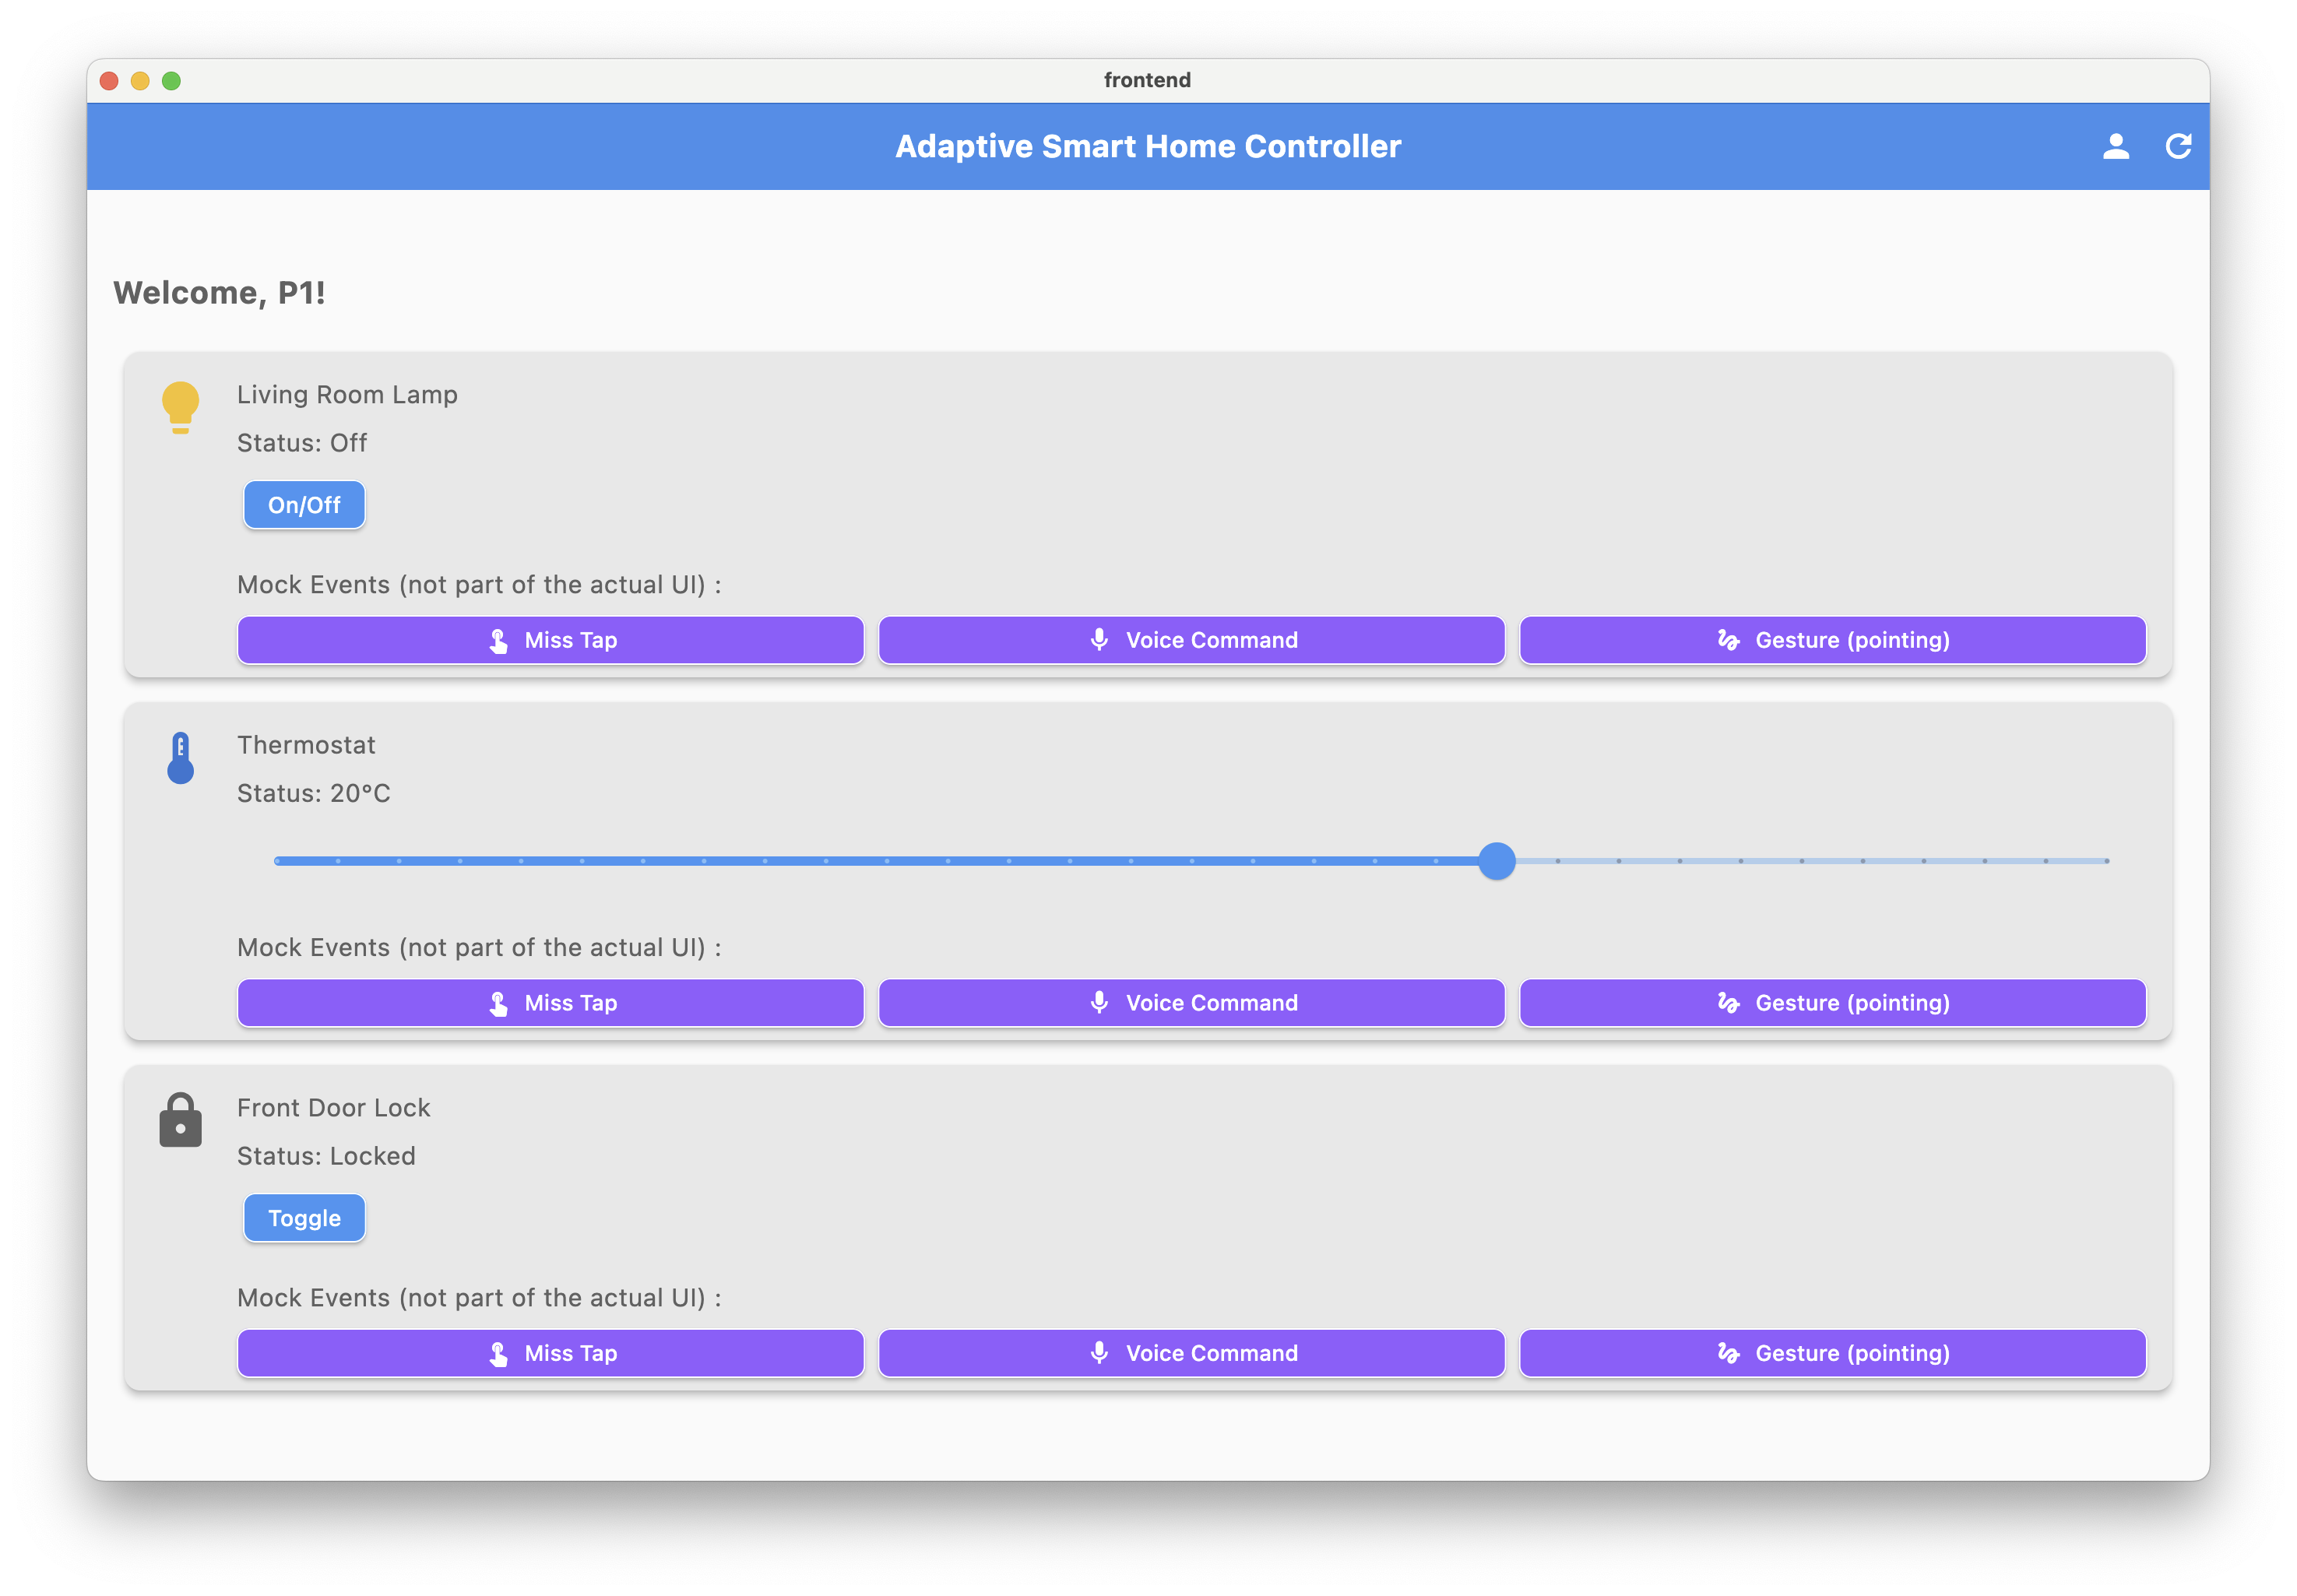
\includegraphics[width=\linewidth]{images/microcase_p1_before.png}\\[-0.5em]
  \centering\small Before (P1, lamp)
\end{minipage}\hfill
\begin{minipage}{0.48\textwidth}
  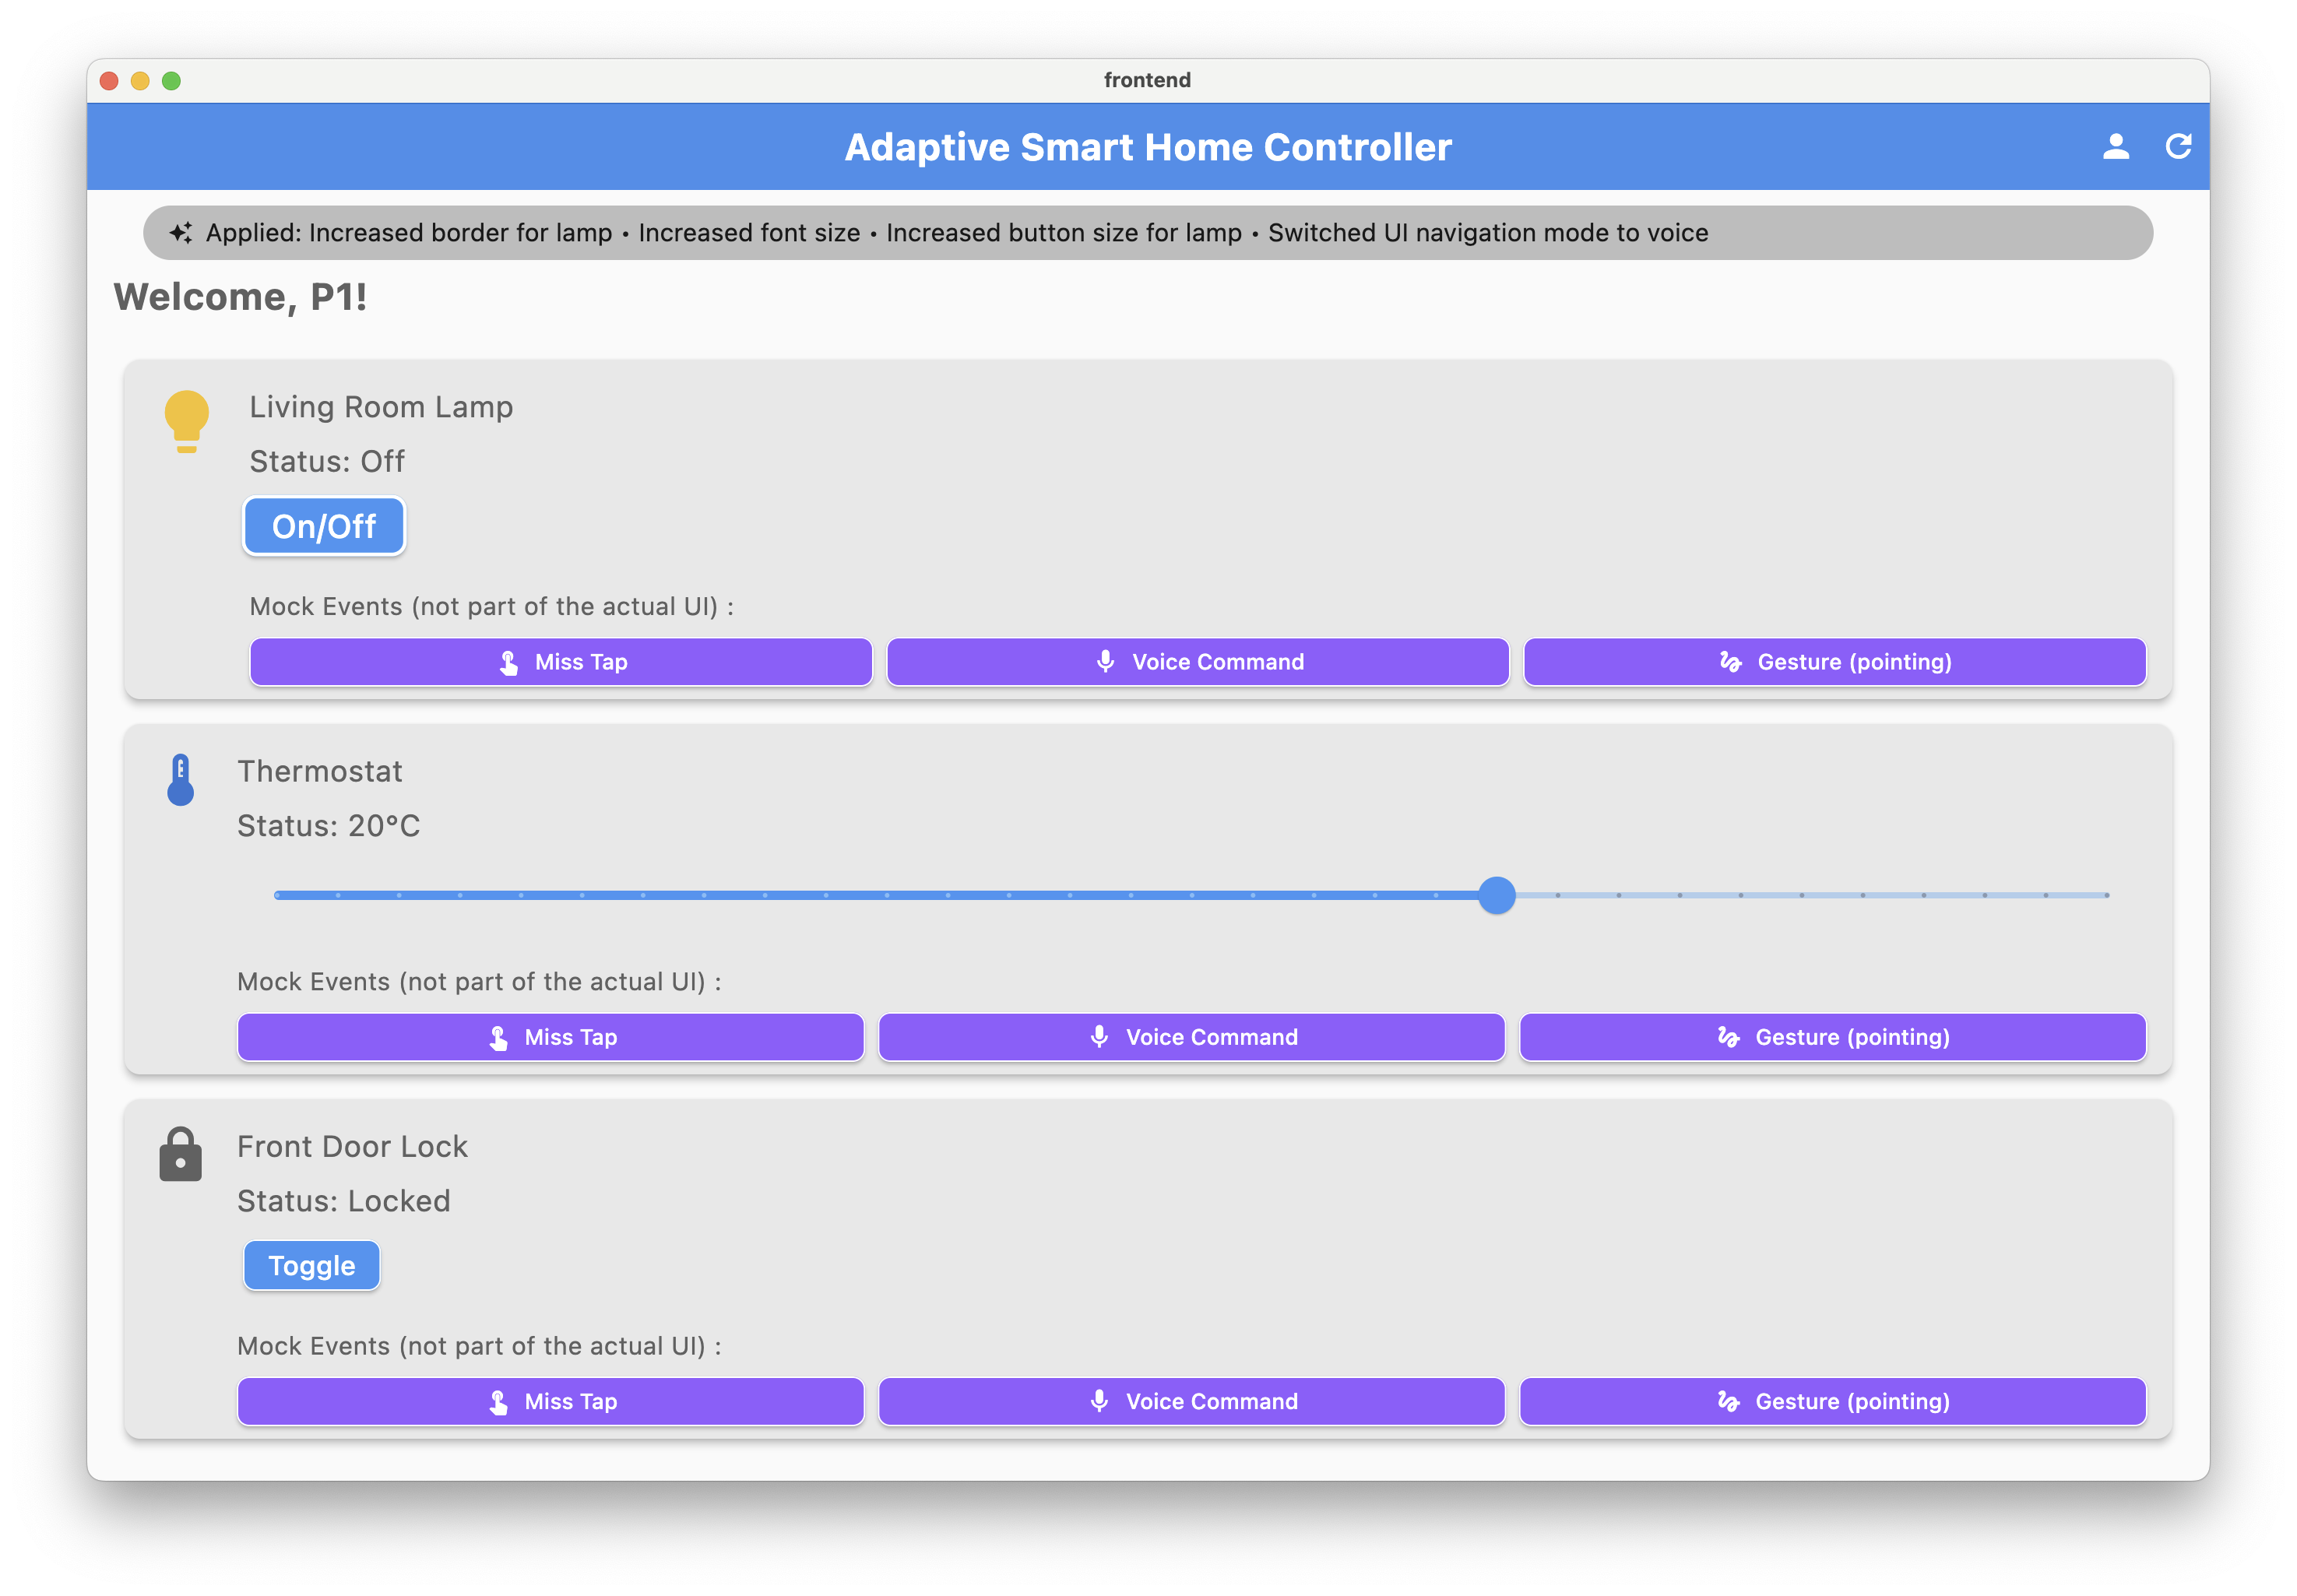
\includegraphics[width=\linewidth]{images/microcase_p1_after.png}\\[-0.5em]
  \centering\small After: larger button and border
\end{minipage}
\caption{P1 (motor) miss\_tap. The adaptation enlarges the button and border, reducing target difficulty. This aligns with P1’s needs and with the objective scores in Table~\ref{tab:obj-metrics} (PAA~50.88\%, ERA~57.14\%, DCI~0.986).}
\label{fig:micro-p1}
\end{figure}

\begin{figure}[H]
\centering
\begin{minipage}{0.48\textwidth}
  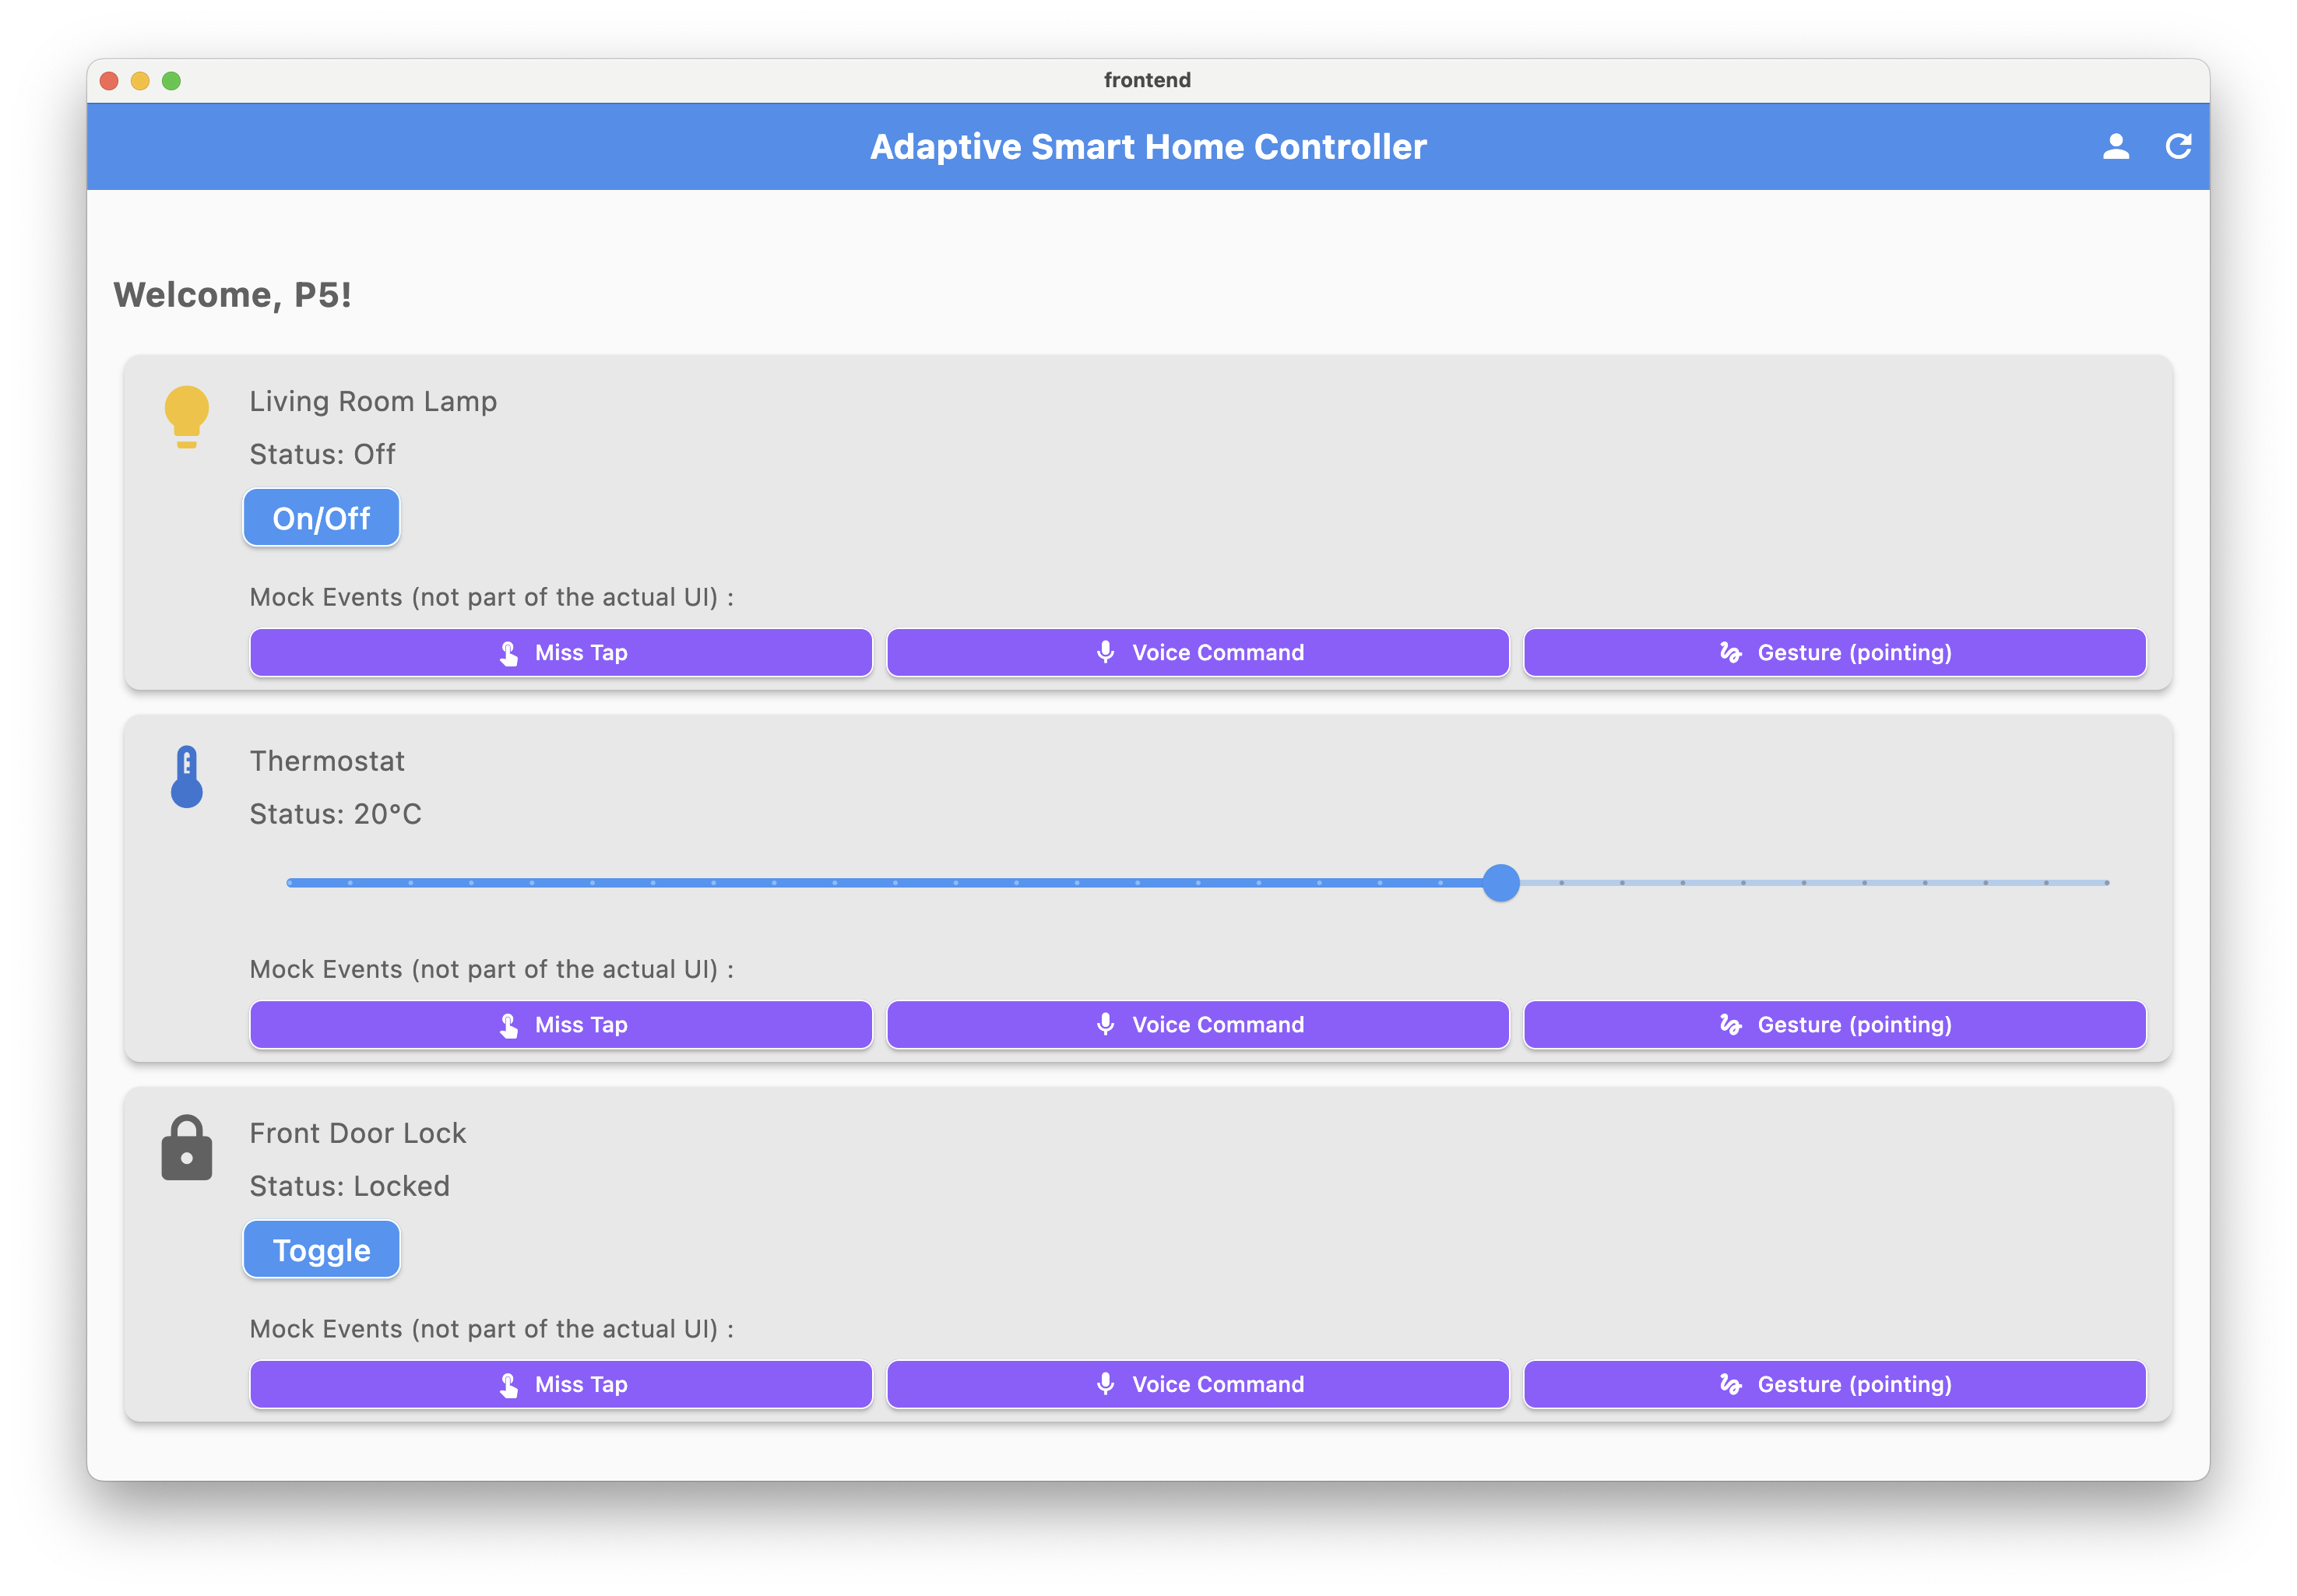
\includegraphics[width=\linewidth]{images/microcase_p5_before.png}\\[-0.5em]
  \centering\small Before (P5, thermostat)
\end{minipage}\hfill
\begin{minipage}{0.48\textwidth}
  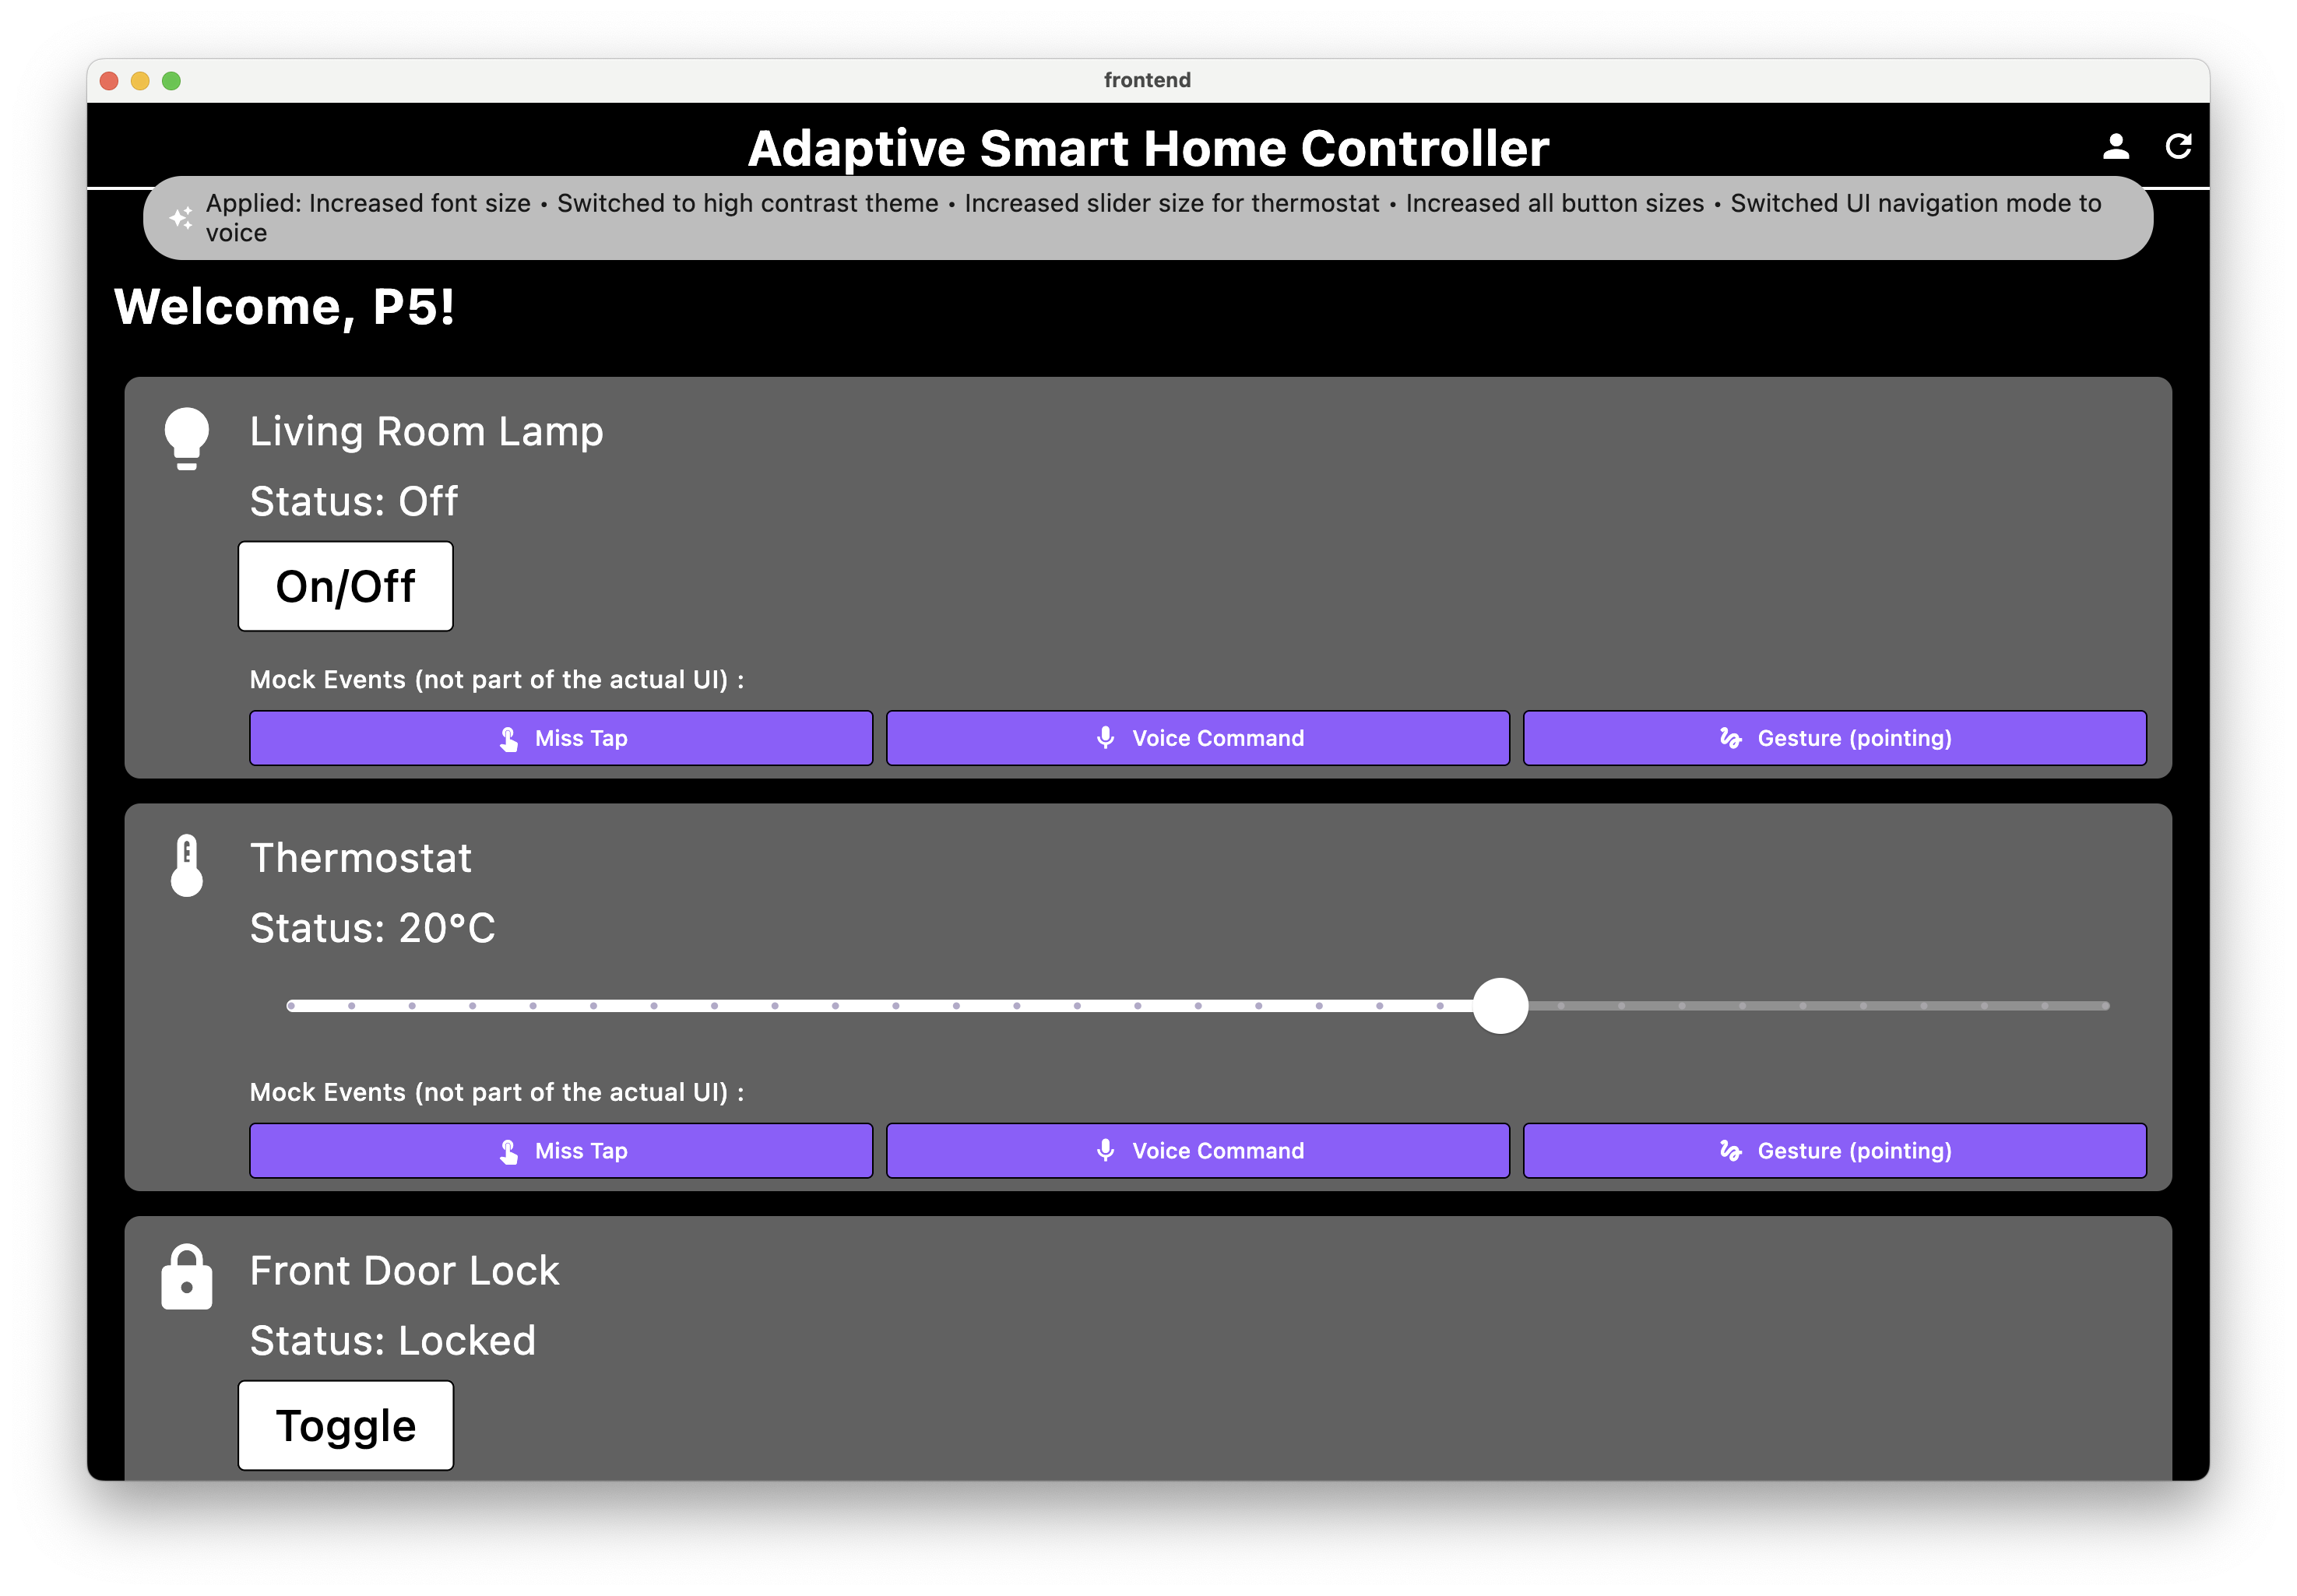
\includegraphics[width=\linewidth]{images/microcase_p5_after.png}\\[-0.5em]
  \centering\small After: larger slider and higher contrast text
\end{minipage}
\caption{P5 (visual+motor) slider\_miss. The adaptation increases slider size, text contrast and more as seen by the notification in the app. This matches P5’s mixed needs and the strong scores in Table~\ref{tab:obj-metrics} (PAA~77.42\%, ERA~64.29\%, DCI~1.000).}
\label{fig:micro-p5}
\end{figure}

\newpage
\section{Adaptation Performance (Latency)}
\label{sec:latency}
Latency is reported separately from accessibility and design quality to avoid conflation of speed with effectiveness. The same MA-SIF (balanced) configuration and client-side $\Delta t$ are used.

\subsection{Overall summary}
Across 84 events and six profiles (Table~\ref{tab:overall-feasibility}):
\begin{itemize}
  \item \textbf{Schema-valid outputs:} 84.52\% of events,
  \item \textbf{Classification path:} 100\% via Validator,
  \item \textbf{Latency:} p50 13.19 s, p90 17.13 s, max 21.10 s.
\end{itemize}

\begin{table}[H]
\centering
\caption{Overall feasibility results with MA-SIF (balanced).}
\label{tab:overall-feasibility}
\begin{tabular}{lr}
\toprule
\textbf{Metric} & \textbf{Value} \\
\midrule
Events (total) & 84 \\
Users (total) & 6 \\
Schema-valid outputs (\%) & 84.52 \\
Validated by Validator (\%) & 100.00 \\
Latency $p_{50}$ (s) & 13.19 \\
Latency $p_{90}$ (s) & 17.13 \\
Latency max (s) & 21.10 \\
\bottomrule
\end{tabular}
\end{table}

The most frequent actions were:
\begin{itemize}
    \item \texttt{switch\_mode} (87): often recommending voice mode.
    \item \texttt{increase\_button\_size} (74), \texttt{increase\_button\_border} (69), \texttt{increase\_font\_size} (66).
    \item \texttt{increase\_slider\_size} (28), \texttt{increase\_contrast} (19).
    \item Less frequent: \texttt{trigger\_button} (9), \texttt{adjust\_spacing} (9).
\end{itemize}
Because multiple suggestions can be attached to one event, action counts exceed the number of events. Top targets were the lamp, thermostat, and lock, with miss-taps most often on lamp and lock (by design).

\paragraph{Interpretation:} The system strongly prioritizes motor-related support (larger targets, borders, spacing) and modal switching to voice when it detects tap/slider errors, exactly the pattern that is needed for motor-impaired and hands-free users. Vision-related support (font size and contrast) also appears consistently, but is less prominent than motor support in this trace.


\subsection{Per profile outcomes}
Validity and latency per profile are in Table~\ref{tab:per-profile}. Latency sits in the 11.8–16.0 s p50 band, with a predictable tail.

\begin{table}[H]
\centering
\caption{Per profile schema validity and latency under MA-SIF (balanced).}
\label{tab:per-profile}
\begin{tabular}{l l r r r r}
\toprule
\textbf{Profile} & \textbf{Declared needs} & \textbf{Valid (\%)} & \textbf{$p_{50}$ (s)} & \textbf{$p_{90}$ (s)} & \textbf{max (s)} \\
\midrule
P0 & Baseline & 78.57 & 16.02 & 20.23 & 21.10 \\
P1 & Motor & 85.71 & 13.19 & 16.78 & 17.43 \\
P2 & Visual & 85.71 & 13.65 & 16.46 & 19.04 \\
P3 & Hands free & 71.43 & 11.82 & 14.68 & 16.49 \\
P4 & Motor + Hands free & 85.71 & 13.63 & 15.76 & 17.91 \\
P5 & Visual + Motor & 100.00 & 12.70 & 16.25 & 16.60 \\
\bottomrule
\end{tabular}
\end{table}

\paragraph{Observations:}
\begin{itemize}
    \item Highest validity appears for combined needs (P5), likely because the event suite provides strong, consistent signals (miss-taps + slider overshoot) that align with the rules and model prior for motor/visual support.
    \item Lowest validity is P3 (hands-free) at 71.43\%. Even though P3 shows the best latency, hands-free preference alone may result in fewer structural UI changes (e.g., fewer size/contrast edits), and the Validator may reject marginal suggestions more often. This indicates room to enrich the hands-free policy (e.g., more explicit voice/gesture affordances and confirmation prompts).
    \item Latency is in the 11.8--16.0 s p50 band across profiles under the MA-SIF (balanced) config. The spread between p50 and p90 ($\approx 3$--$4\,\mathrm{s}$) suggests predictable tail behavior, with a single global max near 21 s.
\end{itemize}

\subsection{Configuration comparison (all profiles)}
For clarity, \emph{Config~A} denotes \textbf{MA-SIF (balanced)} and \emph{Config~B} denotes \textbf{MA-SIF (heavy)}. The comparison aggregates all six profiles (P0–P5) across both runs. Table~\ref{tab:cfg-compare-overall} reports overall latency and quality, and Table~\ref{tab:cfg-compare-profiles} breaks results down by profile.

\begin{table}[ht]
\centering
\caption{Overall configuration comparison (lower latency is better; higher Schema-valid, PAA, ERA, and DCI are better).}
\label{tab:cfg-compare-overall}
\begin{tabular}{lrrrrr}
\toprule
\textbf{Config} & \textbf{p50 (s)} & \textbf{Schema-valid (\%)} & \textbf{PAA (\%)} & \textbf{ERA (\%)} & \textbf{DCI} \\
\midrule
MA-SIF (balanced) & 13.19 & 84.52 & 55.22 & 97.62 & 0.99 \\
MA-SIF (heavy)    & 36.06 & 100.00 & 61.45 & 98.81 & 1.00 \\
\bottomrule
\end{tabular}
\end{table}

\begin{table}[ht]
\centering
\caption{Per-profile configuration comparison (p50 latency, Schema-valid, PAA, ERA, and DCI).}
\label{tab:cfg-compare-profiles}
\begin{tabular}{l l r r r r r}
\toprule
\textbf{Profile} & \textbf{Config} & \textbf{p50 (s)} & \textbf{Schema (\%)} & \textbf{PAA (\%)} & \textbf{ERA (\%)} & \textbf{DCI} \\
\midrule
P0 & MA-SIF (balanced) & 16.02 & 78.57 & 0.00  & 100.00 & 0.98 \\
P0 & MA-SIF (heavy)    & 34.42 & 100.00 & 0.00  & 100.00 & 0.99 \\
P1 & MA-SIF (balanced) & 13.19 & 85.71  & 50.88 & 100.00 & 0.99 \\
P1 & MA-SIF (heavy)    & 34.92 & 100.00 & 65.31 & 100.00 & 0.99 \\
P2 & MA-SIF (balanced) & 13.65 & 85.71  & 34.69 & 85.71  & 1.00 \\
P2 & MA-SIF (heavy)    & 36.55 & 100.00 & 40.98 & 92.86  & 1.00 \\
P3 & MA-SIF (balanced) & 11.82 & 71.43  & 28.00 & 100.00 & 1.00 \\
P3 & MA-SIF (heavy)    & 34.67 & 100.00 & 29.17 & 100.00 & 1.00 \\
P4 & MA-SIF (balanced) & 13.63 & 85.71  & 80.00 & 100.00 & 1.00 \\
P4 & MA-SIF (heavy)    & 40.75 & 100.00 & 100.00& 100.00 & 1.00 \\
P5 & MA-SIF (balanced) & 12.70 & 100.00 & 77.42 & 100.00 & 1.00 \\
P5 & MA-SIF (heavy)    & 38.54 & 100.00 & 77.05 & 100.00 & 1.00 \\
\bottomrule
\end{tabular}
\end{table}

\paragraph{Interpretation.}
MA-SIF (heavy) improves Schema-valid output (100.00\% vs 84.52\%) and raises PAA (61.45\% vs 55.22\%), with small gains in ERA and a near-perfect DCI, at the cost of much higher latency (36.06\,s vs 13.19\,s, about 2.7$\times$ slower). Gains are most visible for P1 and P4 where motor and hands free needs dominate; P5 remains similar, and P3 increases only slightly. In practice, the balanced setting is suitable for interactive adaptation, while the heavy setting is better for post-interaction or batch adaptation where stronger alignment and stricter validation justify the extra delay.

\section{Discussion of Results}
\label{sec:discussion_eval}

\paragraph{Effectiveness.}
The system focuses almost entirely on accessibility: \textbf{97.51\%} of all actions are accessibility targeted (Table~\ref{tab:overall-accessible-share}). Internal coherence is high across profiles (\textbf{DCI} $\approx$ \textbf{0.995}; Table~\ref{tab:obj-metrics}). Appropriateness is strong for motor and voice inputs: \texttt{miss\_tap} and \texttt{slider\_miss} reach \textbf{100\%} ERA and \texttt{voice} \textbf{97.22\%}, while \texttt{gesture} remains low at \textbf{8.33\%} (Table~\ref{tab:era-by-event}). In the configuration comparison, MA-SIF (heavy) reaches \textbf{100.00\%} schema-valid outputs and slightly higher ERA and DCI than the balanced setting (Table~\ref{tab:cfg-compare-overall}), confirming that stricter aggregation and checking can push quality to the top end.

\paragraph{Personalization.}
Profile–Action Alignment (PAA) is moderate overall (\(\sim\)\textbf{55\%} on top–5 actions) and higher for combined-need profiles (P4, P5), which matches the event suite that emphasises motor errors and mode switching (Table~\ref{tab:obj-metrics}). MA-SIF (heavy) increases PAA from \textbf{55.22\%} to \textbf{61.45\%} overall (Table~\ref{tab:cfg-compare-overall}) and produces the largest gains where motor and hands free needs dominate (P1, P4; Table~\ref{tab:cfg-compare-profiles}). Some potential improvements include:
\begin{enumerate}
  \item \textbf{Weighted validator scoring:} Rank candidates higher when their category matches the active need, and apply gentle penalties for off-need actions.
  \item \textbf{Lightweight feedback signals:} Log accept, undo, and reversion in the client and feed these rates back as simple weights to prefer actions users keep.
  \item \textbf{Richer hands free affordances:} Add confirmation prompts, focus hints, and voice-first navigation so that acceptable sets are available more often, lifting both ERA and PAA for hands free profiles.
\end{enumerate}

\paragraph{Latency.}
MA-SIF (balanced) achieves a median of \textbf{13.19\,s} versus \textbf{36.06\,s} for MA-SIF (heavy) (Table~\ref{tab:cfg-compare-overall}). The balanced path is more suitable for interactive adaptation, while the heavy path offers stricter outputs for post-interaction or batch contexts. The rule-only sufficiency proxy in Section~\ref{sec:era-by-event} and the fast-path analysis indicate that \(\sim\)\textbf{86\%} of events contain at least one corrective action that a simple rule can provide. A staged design is therefore practical: route obvious patterns directly through a rule path and keep the Validator for consolidation, while leaving ambiguous or gesture-driven events to full multi-agent reasoning.

\section{Study Limitations}
\begin{itemize}
  \item \textbf{Feasibility focus.} The evaluation uses structured traces; no human-subject (user) study is included.
  \item \textbf{Trace coverage.} The suite is representative but not exhaustive; real use may show different dwell and timing patterns.
  \item \textbf{Configuration scope.} Two configurations are compared (balanced and heavy). Other variants (for example single-agent SIF or different model budgets) are not explored here.
  \item \textbf{Action menu scope.} The allowed actions form a compact, WCAG-oriented set. This is developer realistic, but it may bias coverage toward needs with generic remedies and does not balance action counts across profiles.
  \item \textbf{Validator transparency.} Rejection reasons are not logged by design, which limits a fine-grained taxonomy of invalid cases; client-side schema checks are used instead.
  \item \textbf{Environment.} Results reflect a single-machine setting with Gemini API calls; other deployments may shift latency.
\end{itemize}

\section{Conclusion}
The framework delivers valid, accessibility-focused, and coherent adaptations. Objective metrics in Section~\ref{sec:objective-quality} show strong accessibility focus and high internal coherence, with moderate personalization that improves under the heavier configuration. The configuration comparison (Tables~\ref{tab:cfg-compare-overall} and~\ref{tab:cfg-compare-profiles}) makes the trade-off explicit: MA-SIF (heavy) raises schema validity and PAA at a substantial latency cost, while MA-SIF (balanced) keeps latency acceptable for asynchronous interaction. The analyses by event type and run stability indicate clear next steps: add need-weighted validator scoring, integrate lightweight user feedback, and extend hands free affordances. These directions increase personalization and keep the schema-based, reproducible evaluation intact, strengthening the case for multimodal, AI-driven adaptation in real-world interfaces.